\shorthandoff{<>}
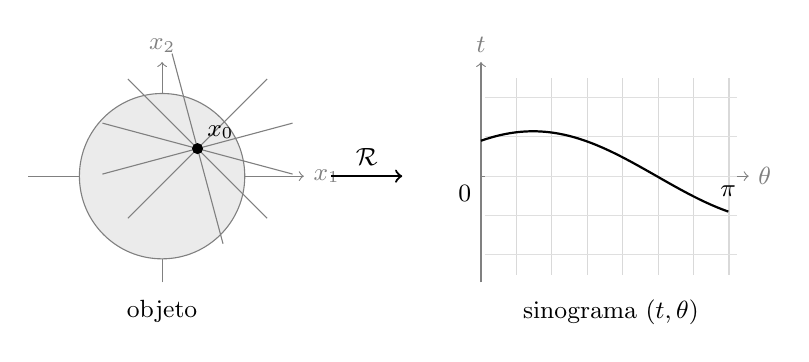
\begin{tikzpicture}[font=\small]
    \begin{scope}
        \draw[->, thin, gray] (-1.7,0) -- (1.8,0) node[right] {$x_1$};
        \draw[->, thin, gray] (0,-1.35) -- (0,1.45) node[above] {$x_2$};
        \draw[fill=black!8, draw=black!50] (0,0) circle (1.05);
        \coordinate (Xzero) at (0.45,0.35);
        \foreach \a in {15,45,75,105,135} {
            \draw[thin, gray] (Xzero) ++(\a+90:1.25) -- ++(\a-90:2.5);
        }
        \fill (Xzero) circle (2pt) node[above right] {$x_0$};
        \node[below] at (0,-1.45) {objeto};
    \end{scope}

    \draw[->, thick] (2.15,0) -- (3.05,0) node[midway, above] {$\mathcal R$};

    \begin{scope}[xshift=4.05cm]
        \draw[->, thin, gray] (0,0) -- (3.4,0) node[right] {$\theta$};
        \draw[->, thin, gray] (0,-1.35) -- (0,1.45) node[above] {$t$};
        \foreach \x in {0.45,0.9,...,3.15} {
            \draw[thin, gray!30] (\x,-1.25) -- (\x,1.25);
        }
        \foreach \y in {-1.0,-0.5,0,0.5,1.0} {
            \draw[thin, gray!25] (0.05,\y) -- (3.25,\y);
        }
        \draw[thick, black, domain=0:3.1416, samples=80, variable=\u]
            plot ({\u}, {0.45*cos(\u r)+0.35*sin(\u r)});
        \node[below left] at (0,0) {$0$};
        \node[below] at (3.14,0) {$\pi$};
        \node[align=center, below] at (1.65,-1.45) {sinograma $(t,\theta)$};
    \end{scope}
\end{tikzpicture}
\shorthandon{<>}
